%%%%%%%%%%%%%%%%%%%%%%%%%%%%%%%%%%%%%%%%%%%%%%%%%%%%%%%%%%%%%%%%%%%%%%%
%%%%  Load the document class and packages                         %%%%
%%%%%%%%%%%%%%%%%%%%%%%%%%%%%%%%%%%%%%%%%%%%%%%%%%%%%%%%%%%%%%%%%%%%%%%
\documentclass[a4paper]{report}
\usepackage{epsfig}            % to insert PostScript figures
\graphicspath{
	{./figures/}
}

%Change figure names
\renewcommand{\figurename}{Fig}

\usepackage[bf,footnotesize]{caption} % make captions small and label bold

\addtocounter{chapter}{1} %Because starting at zero is silly
\makeatletter
\renewcommand{\thesection}{\@arabic\c@section}
\renewcommand{\thefigure}{\@arabic\c@figure}
\makeatother

\usepackage{titlesec} %change spacing before and after sections
%format: \titlespacing*{<command>}{<left>}{<before-sep>}{<after-sep>}
\titlespacing*{\section}{0pt}{11mm plus 1ex minus .2ex}{6mm plus .2ex}
\titlespacing*{\subsection}{0pt}{9mm plus 1ex minus .2ex}{4mm plus .2ex}

\usepackage[a4paper,margin=3.7cm,tmargin=2.5cm,bmargin=2.5cm]{geometry}
\usepackage{textcomp}          % To make nice degree symbols and others
\usepackage[bf,footnotesize]{caption} % make captions small and label bold
\usepackage{wrapfig}
%to produce the clickable references along the left in Acroread. This
%package must be included last.
\usepackage[ps2pdf,bookmarks=TRUE]{hyperref}
\hypersetup{
    colorlinks=true,
    linkcolor=cyan,
    filecolor=magenta,
    urlcolor=cyan,
}

%%%%%%%%%%%%%%%%%%%%%%%%%%%%%%%%%%%%%%%%%%%%%%%%%%%%%%%%%%%%%%%%%%%%%%%
%%%%  Hypertext references for Acrobat                             %%%%
%%%%%%%%%%%%%%%%%%%%%%%%%%%%%%%%%%%%%%%%%%%%%%%%%%%%%%%%%%%%%%%%%%%%%%%
\hypersetup{
	pdfauthor = {SWC},
	pdftitle = {Optics Exercises: Kohler},
	pdfkeywords = {optics, lenses, refraction, reflection, dispersion,
		telescope, microscope},
	pdfcreator = {LaTeX with hyperref},
}

%%%%%%%%%%%%%%%%%%%%%%%%%%%%%%%%%%%%%%%%%%%%%%%%%%%%%%%%%%%%%%%%%%%%%%%
%%%%  Main text                                                    %%%%
%%%%%%%%%%%%%%%%%%%%%%%%%%%%%%%%%%%%%%%%%%%%%%%%%%%%%%%%%%%%%%%%%%%%%%%
\begin{document}

%set the number of sectioning levels
\setcounter{secnumdepth}{2}

\begin{center}
	\textbf{\Large{Brightfield Illumination}}
\end{center}


\vspace{0.8cm}
\noindent
The goal of this demo is to get you more familiar with brightfield microscopy, K\"{o}hler illumination, and how an image is formed via diffraction. 

%%%%%%%%%%%%%%%%%%%%%%%%%%%%%%%%%%%%%%%%%%%%%%%%%%%%%%%%%%%%%%%%%%%%%%%
\section{Illuminating the sample}
%%%%%%%%%%%%%%%%%%%%%%%%%%%%%%%%%%%%%%%%%%%%%%%%%%%%%%%%%%%%%%%%%%%%%%%
\hypertarget{hintBack-illumination}{}
In a transmission illumination light microscope, the illumination of the sample should be 1) bright, 2) uniform, and 3) angled. In addition, we need control over the 4) field of illumination, 5) angles of illumination, and 6) brightness of illumination.
These aims are achieved by K\"{o}hler illumination:

\begin{figure}[h]
	\center
	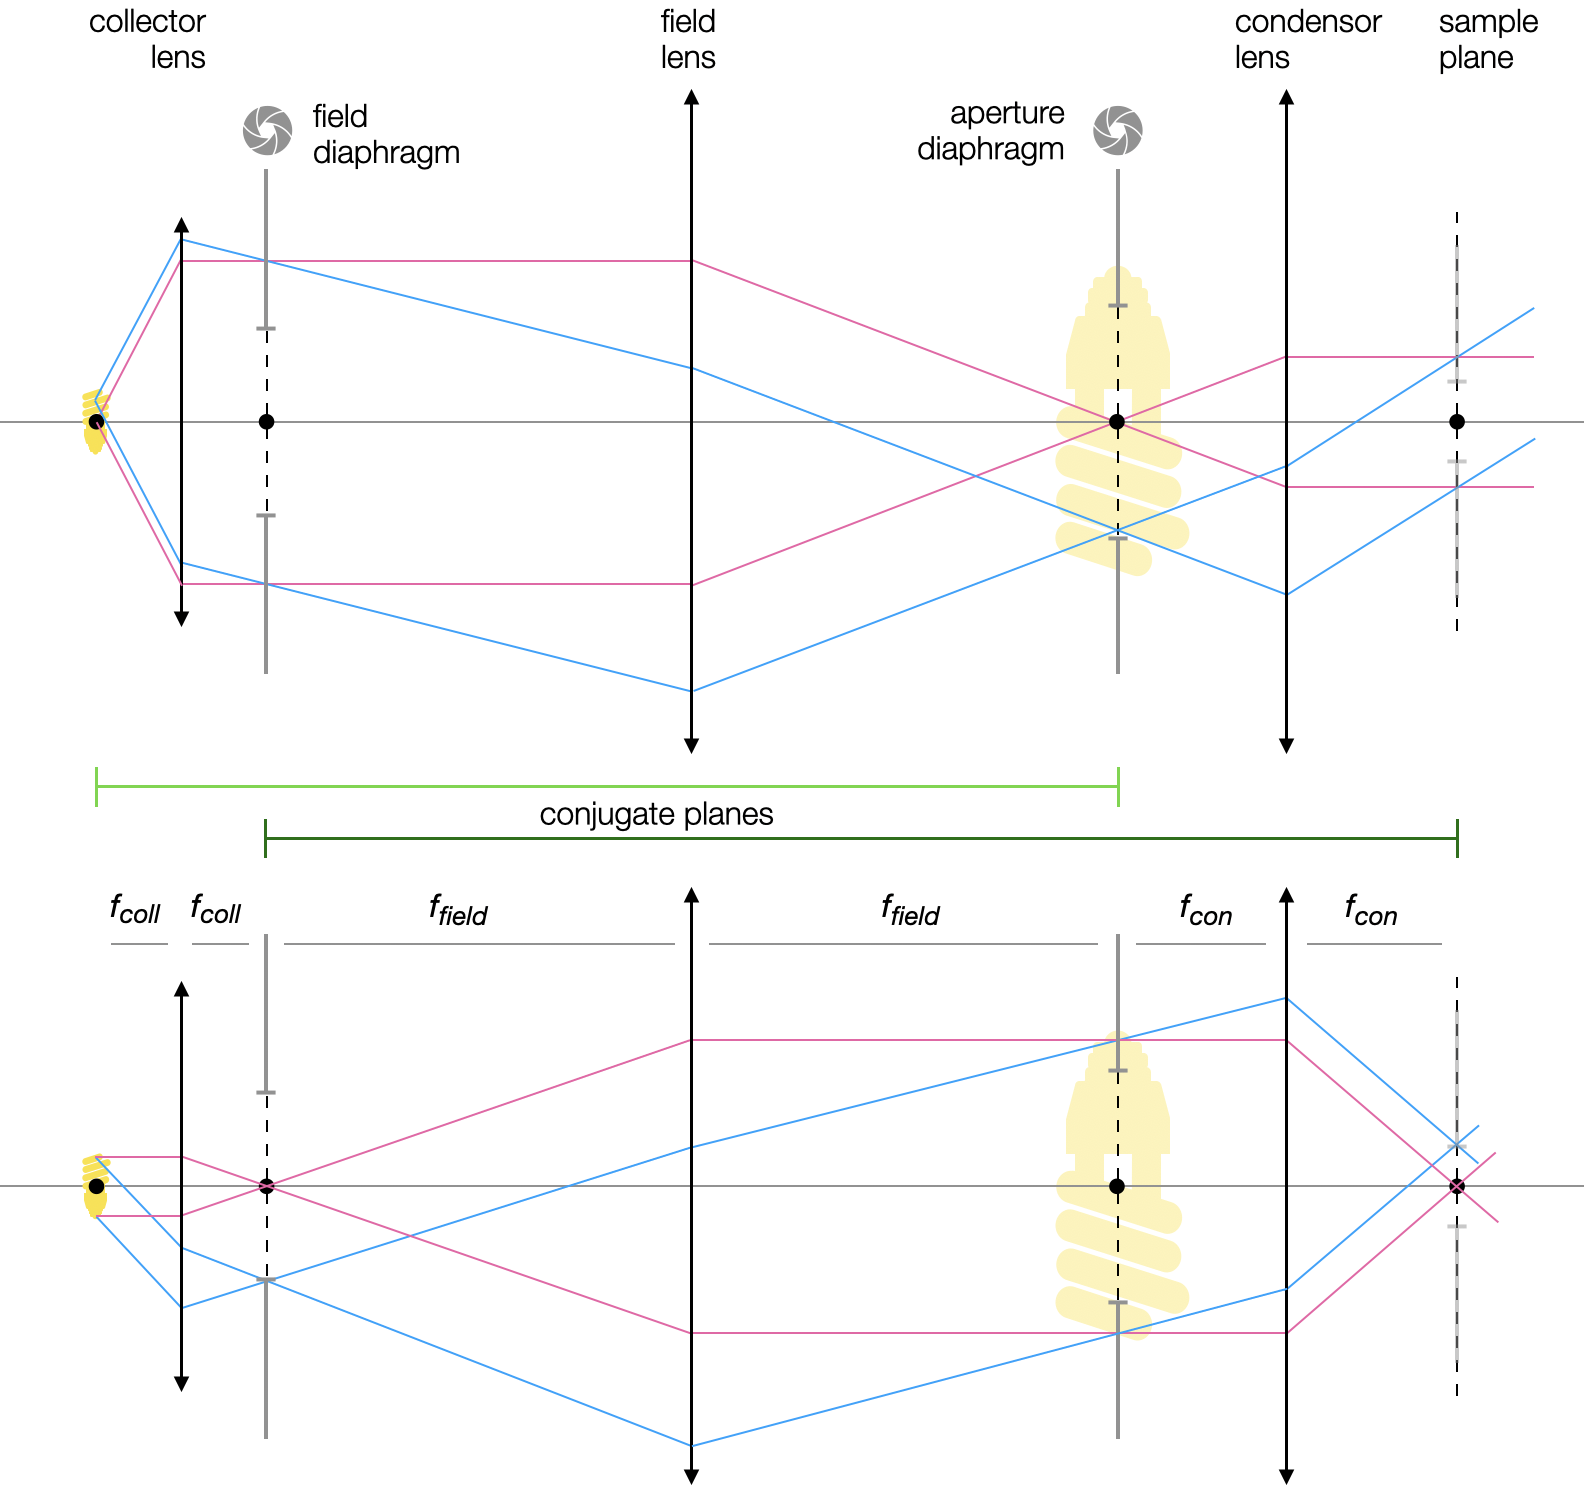
\includegraphics[width=1\textwidth]{figures/koehler_illumination.png}
	\captionsetup{width=0.95\textwidth}
	\caption{K\"{o}hler illumination. \\
	\emph{Top:} Rays are drawn highlighting the infinite conjugate formed by collector and field lens. These rays illustrate i) how each point on the light source illuminates the whole sample, yielding uniform illumination; ii) how the light source is imaged onto the aperture diaphragm with $m=f_{field}/f_{coll}$ (here $m=-5$); iii) how closing the aperture diaphragm shrinks the effective extent of the light source, and hence the angles with which the sample is illuminated, but has no effect on the area of the sample that is illuminated. \\
	\emph{Bottom:} Rays are drawn highlighting the infinite conjugate formed by field and condensor lens. These rays illustrate i) how each point on the sample receives light from all points on the light source; ii) how the field diaphragm is imaged onto the sample plane with $m=f_{con}/f_{field}$ (here m=-2.5); iii) how closing the field diaphragm restricts the area on the sample that is illuminated, but has no effect on the angles of illumination.}
	\label{fig:koehler_illumination}
\end{figure}


\subsection{The K\"{o}hler Illumination Demo}
You will go through a guided demo of K\"{o}hler illumination with the TAs. 
We have pre-assembled the system out of ThorLabs parts so you can follow the optical path and see how the irises affect depth of field of and field of view.
The demo will showcase the features of K\"{o}hler illumination:

\begin{enumerate}
    \item Bright: You can see that the higher the numerical aperture (NA) of the collector lens, the more light is collected from the LED. $NA=sin(a)$, where $a$ is the half-angle of the maximal cone of light the lens can `collimate' (example: a $50mm$ diameter lens with $f=25mm$ has an $NA=45deg$).
    \item Uniform: Only if the illumination is uniform can we attribute differences in brightness in the image to the structure in the sample. How do we avoid seeing the shape of the light source on the sample? We make sure the light source is `de-focused' on the sample, meaning it is imaged to infinity in the sample plane. The top panel in Fig. \ref{fig:koehler_illumination} illustrates this: each point on the light source illuminates the whole sample.
    \item Angled: This has to do with diffraction orders. Light falling onto the sample diffracts, with finer spatial detail leaving the sample at larger angles. Therefore, the resolution of our imaging system (objective and tube lens) is higher the more angles it can accept - we `reconstruct' the sample using more fine-grained spatial information. Only the zero and first order needs to be captured by the objective (additional orders just increase brightness, but carry no further information about the spatial features contained in that angle). As a consequence, an additional way to increase the resolution of the system is to use angled illumination: this rotates the diffraction orders by the same amount as the illumination, making the zero orders fall away from the centre of the objective. This can effectively double the widest acceptable angle between the zero and first order, if the illumination contains angles of at least the acceptance angle of the objective lens, thus doubling resolution. Under these circumstances, the abbe resolution criterion $\lambda / (2\cdot NA)$ holds.
    \item Control over field of illumination: Light falling on regions of the sample outside of what is imaged by the camera sensor is to be avoided for two reasons. First, it might damage the sample unnecessarily; Second, and more importantly, it can scatter within the sample and enter the objective, not having diffracted from within the imaged area and therefore decreasing contrast (signal to noise so to speak) in the image.
    \item Control over angles: This again relates to diffraction orders and is useful for three reasons. First, from the argument in point 3. follows that illuminating the sample with more extreme angles than given by the NA of the objective does nothing to increase resolution. Therefore, that light is better blocked with the aperture diaphragm to avoid decreasing contrast, for the same reasons given in point 4. Second, while we always want maximal $xy$-resolution, $z$-resolution is not always desirable. High $z$-resolution means a shallow \emph{depth-of-field}, where objects are in focus in a narrow optical plane only -- this means many features will appear blurred on the sensor (unless the sample is cut very thinly). Closing the aperture diaphragm will decrease $z$-resolution, thereby increasing the depth-of-field. Third, see point 6.
    \item Control over brightness: If xy-resolution is not a major concern, closing the aperture allows for control of the intensity of illumination -- it affects all points in the sample equally, reducing the angles of illumination and thus dimming the illumination.
\end{enumerate}

\pagebreak


%%%%%%%%%%%%%%%%%%%%%%%%%%%%%%%%%%%%%%%%%%%%%%%%%%%%%%%%%%%%%%%%%%%%%%%
\section{How images are really formed}
%%%%%%%%%%%%%%%%%%%%%%%%%%%%%%%%%%%%%%%%%%%%%%%%%%%%%%%%%%%%%%%%%%%%%%%
\subsection{Modern microscope objectives}
As you learned previously, a single lens is sufficient to form an image. 
This is how cameras, eyes, and telescopes work. 
However, modern microscopes use an infinite conjugate lens \textit{pair} to form an image. 
A major reason for this is resolution: the larger the acceptance angle or $NA$ of the objective lens collecting the diffraction orders from the sample, the higher the resolution (or the more faithful the reconstruction of the sample). 
Whilst using a single lens is possible, the sample would have to be placed between $-2f$ and $-1f$ -- this decreases the effective NA of the lens (can you see why?).
Adding the second lens (the so-called `tube lens') allows the objective to be placed at $-1f$. 
Magnification can be changed by using objectives with different focal lengths, whilst the tube lens remains fixed. 

\subsection{The Fourier plane}
The sample is placed at $-1f$ (the objective front focal plane) of the objective lens and so an image is formed at infinity.
The so-called Fourier plane occurs at $+1f$, which is the objective back (rear) focal plane. 
It is at this point that a Fourier transform of the object plane can found.
The Fourier plane can be treated as an object and imaged onto a camera. 
However, under normal circumstances, the Fourier transform itself is not visible. 
In real samples the Fourier transform is very complicated and is obscured by the way samples are illuminated and the fact that they are 3D.

\subsubsection{Visualising the Fourier plane}
Today you will see see the the simple Fourier transforms of carefully illuminated synthetic samples using a two-camera microscope. One camera shows the image of the sample using a tube lens as normal.
A beam splitter cube adds a second camera that simultaneously images the Fourier plane.
A variable slit is placed at the Fourier plane allowing us to selectively block different components and observe how this affects the image. 
You will see how removing specific higher frequencies blurs the image in predictable ways. 
Using a coloured filter wheel you will also see how shorter wavelengths are diffracted more by the objective and so produce images of higher resolution.   

\pagebreak


%%%%%%%%%%%%%%%%%%%%%%%%%%%%%%%%%%%%%%%%%%%%%%%%%%%%%%%%%%%%%%%%%%%%%%%
\section{Imaging the sample}
%%%%%%%%%%%%%%%%%%%%%%%%%%%%%%%%%%%%%%%%%%%%%%%%%%%%%%%%%%%%%%%%%%%%%%%


We will now build the imaging side of a microscope using a high quality objective lens and use this to visualise Golgi stained neurons.

\subsection{What is a microscope objective lens?}
%----------------------------------------------------------------------
Microscope objectives are designed to work in the infinite conjugate configuration with another lens: they are `infinity corrected'.
This means that aberrations (chromatic and spherical, usually) are maximally corrected for in the focal plane, away from which they will swiftly increase.
It stands to reason that the 4x objective in your kit magnifies an object 4x \emph{given a second lens with a particular focal length} (called a tube lens), specific to the manufacturer. Olympus uses $f=180mm$ tube lenses in their microscopes.

\begin{itemize}
    \item Calculate the focal length of the 4x objective. Choose a tube lens and calculate the magnification of your imaging setup.
    
    \item Since objectives are compound lenses, the optical centre is not known to the user, symmetrically around which lie the focal points. The manufacturer instead tells us the `working distance' WD, which is the distance of the focal plane from the tip of the objective; this is where we place the sample. WD can be hard to measure (for instance 0.8~mm) -- how can we ensure our sample is ends up at WD from the tip of the objective when in focus? Hint: think about the whole optical assembly and all the components. 
    \item What do you expect to be able to see with your microscope? A hair (0.1mm)? A neuron (0.01mm)? Mitochondria (0.001mm)?

\end{itemize}
  
   
\subsection{Let's build it}
For simplicity we will illuminate the sample with an LED placed near to the slide and form an image on a screen.

\begin{itemize}
\item Place the white LED on the rail and immediately after it a slide holder.
\item Mount the objective on a post on the other side. The objective needs a special adapter ring: ask a TA if you don't find it right away. 
\item Make sure the tube lens is $f_{tube}$ from the screen and at the same height as the objective. 
\item Place a sample in the holder and produce a focused image on the screen. Remember: you are sliding the objective on the rail for focus. Do not focus by moving the screen.
\item If time allows you can set up a camera.
\end{itemize}
 

%%%%%%%%%%%%%%%%%%%%%%%%%%%%%%%%%%%%%%%%%%%%%%%%%%%%%%%%%%%%%%%%%%%%%%%

\pagebreak
\hypertarget{hintTo-imaging}{}

\subsection{A question of resolution}
When we ask `can we see it?', we think of separating objects of that size from each other. If there are two cells next to each other, will you see two cells?
Abbe tells us if the effective condensor NA equals the objective NA, we can just distinguish things that are $\lambda / (2NA)$ apart.
For the 4x objective ($NA=0.1$) and $500nm$ light, this gives 2.5$\mu m$ -- surprised?
You just built a microscope! Though is your effective condensor $NA\geq 0.1$?
What can you see with the 10x objective?

   \noindent
   \hyperlink{hintBack-imaging}{Go back}

\subsubsection{Ensuring image formation at 1 WD}
If the tube lens is exactly $1f$ away from the camera sensor, we will see the sample in focus when it is at $1f$ from the objective.
Thus, the tube lens--camera distance must be carefully measured, which is doable since a typical tube lens has a focal length of around 200mm.
To bring the sample into focus, the objective can be moved with respect to the sample, making use of the infinite space between objective and tube lens.
If the objective is switched out for a higher power one (with a shorter focal length), nothing changes on our imaging setup except we re-focus on the sample by moving the objective.
\noindent
\hyperlink{hintBack-imaging}{Go back}
\clearpage
\end{document}
